\chapter{Не только списки: другие применения cons-ячеек}
\label{ch:13}

\thispagestyle{empty}

Как вы увидели в предыдущей главе, списочный тип данных является иллюзией, созданной
множеством функций, которые манипулируют cons-ячейками. Common Lisp также предоставляет
функции, позволяющие вам обращаться со структурами данных, созданными из cons-ячеек, как c
деревьями, множествами и таблицами поиска (\textit{lookup tables}). В~этой главе я дам
вам краткий обзор некоторых из этих структур данных и оперирующих с ними функций. Как и в
случае функций, работающих со списками, многие из них будут полезны, когда вы начнёте
писать более сложные макросы, где потребуется обращаться с кодом Lisp как с данными.

\section{Деревья}

Рассматривать структуры, созданные из cons-ячеек, как деревья так же естественно, как
рассматривать их как списки. Ведь что такое список списков, как не другое представление
дерева?  Разница между функцией, которая обращается с группой cons-ячеек как со списком, и
функцией, обращающейся с той же группой cons-ячеек как с деревом, определяется тем, какие
ячейки обходят эти функции при поиске значений для дерева или списка. Те сons-ячейки,
которые обходит функция работы со списком, называются \textit{списочной структурой}
(\textit{list structure}) и
располагаются, начиная от первой cons-ячейки и затем следуя ссылкам по \lstinline{CDR}, пока не
достигнут \lstinline{NIL}.  Элементами списка являются объекты, на которые ссылаются
\lstinline{CAR}'ы cons-ячеек списочной структуры. Если cons-ячейка в списочной структуре имеет
\lstinline{CAR}, который ссылается на другую cons-ячейку, то та ячейка, на которую ведёт
ссылка, считается головой и элементом внешнего списка\footnote{Возможно создать цепь
  списочных ячеек, где \lstinline{CDR} последней ячейки будет не \lstinline{NIL}, а неким другим
  атомом. Такая конструкция будет называться \textit{точечным списком} (\textit{dotted
    list}), потому что последняя списочная ячейка является точечной парой.}.
\textit{Древовидная структура} (\textit{tree structure}), с другой стороны, при обходе следует
ссылкам как по \lstinline{CAR}, так и по \lstinline{CDR}, пока они указывают на другие cons-ячейки. Таким
образом, значениями в древовидной структуре являются атомы~-- такие значения, которые не
являются cons-ячейками и на которые ссылаются \lstinline{CAR}'ы или \lstinline{CDR}'ы cons-ячеек в
древовидной структуре.

Например, следующая стрелочная диаграмма показывает cons-ячейки, составляющие список из
списков: \lstinline{((1 2) (3 4) (5 6))}. Списочная структура включает в себя только три
cons-ячейки внутри пунктирного блока, тогда как древовидная структура включает все ячейки.

\begin{figure}[h]
  \centering
  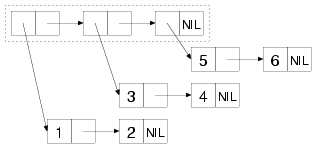
\includegraphics[scale=0.6]{images/list-or-tree.png}
\end{figure}

Чтобы увидеть разницу между функцией, работающей со списком, и функцией, работающей с
деревом, вы можете рассмотреть, как функции \lstinline{COPY-LIST} и \lstinline{COPY-TREE} будут
копировать эту группу cons-ячеек. \lstinline{COPY-LIST} как функция, работающая со списком,
копирует cons-ячейки, которые составляют списочную структуру. Другими словами, она создаёт
новые cons-ячейки соответственно для каждой из cons-ячеек пунктирного блока. \lstinline{CAR}'ы
каждой новой ячейки ссылаются на тот же объект, что и \lstinline{CAR}'ы оригинальных cons-ячеек
в списочной структуре. Таким образом, \lstinline{COPY-LIST} не копирует подсписки
\lstinline{(1, 2)}, \lstinline{(3 4)}, или \lstinline{(5 6)}, как показано на этой диаграмме:

\begin{figure}[h]
  \centering
  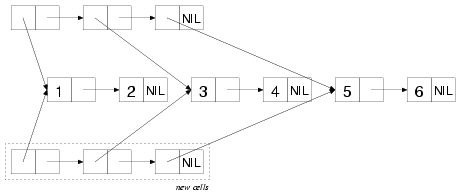
\includegraphics[scale=0.6]{images/copy-list-list-or-tree.png}
\end{figure}

\lstinline{COPY-TREE}, с другой стороны, создаёт новые cons-ячейки для каждой из cons-ячеек на
диаграмме и соединяет их вместе в одну структуру, как показано на рис.~\ref{fig:13-3}.

\begin{figure}[h]
  \centering
  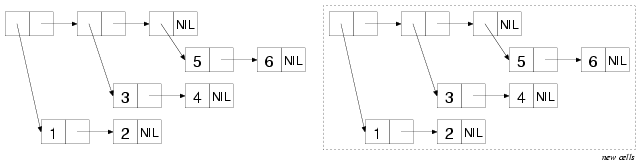
\includegraphics[scale=0.6]{images/copy-tree-list-or-tree.png}
  \caption{Результат использования \lstinline{COPY-TREE}.}
  \label{fig:13-3}
\end{figure}

Там, где cons-ячейки в оригинале ссылаются на атомарное значение, соответствующие им
cons-ячейки в копии будут ссылаться на то же значение.  Таким образом, единственными
объектами, на которые ссылаются как оригинальное дерево, так и его копия, созданная
\lstinline{COPY-TREE}, будут числа \lstinline{5}, \lstinline{6} и символ \lstinline{NIL}.

Еще одна функция, которая обходит как \lstinline{CAR}'ы, так и \lstinline{CDR}'ы cons-ячеек дерева,~--
это \lstinline{TREE-EQUAL}, которая сравнивает два дерева и считает их равными, если их
структуры имеют одинаковую форму и если их листья равны относительно \lstinline{EQL} (или если
они удовлетворяют условию, задаваемому через именованный аргумент \lstinline{:test}).

Прочими ориентированными на деревья функциями являются работающие с деревьями аналоги
функций для последовательностей \lstinline{SUBSTITUTE} и \lstinline{NSUBSTITUTE}, а также их \lstinline{-IF} и
\lstinline{-IF-NOT} варианты. Функция \lstinline{SUBST}, как и \lstinline{SUBSTITUTE}, принимает новый
элемент, старый элемент и дерево (в отличие от последовательности) вместе с именованными
аргументами \lstinline{:key} и \lstinline{:test} и возвращает новое дерево с той же формой, что и
исходное, но все вхождения старого элемента заменяются новым. Например:

\begin{myverb}
CL-USER> (subst 10 1 '(1 2 (3 2 1) ((1 1) (2 2))))
(10 2 (3 2 10) ((10 10) (2 2)))
\end{myverb}

\lstinline{SUBST-IF} аналогична \lstinline{SUBSTITUTE-IF}. Но вместо старого элемента она принимает
одноаргументную функцию, которая вызывается с аргументом в виде каждого атомарного
значения в дереве, и всякий раз, когда она возвращает истину, текущая позиция в новом
дереве заменяется новым значением. \lstinline{SUBST-IF-NOT} действует так же, за исключением
того, что заменяются те значения, где функция возвращает \lstinline{NIL}. \lstinline{NSUBST},
\lstinline{NSUBST-IF}, и \lstinline{NSUBST-IF-NOT}~-- это утилизирующие аналоги соответствующих
версий \lstinline{SUBST}-функций. Как и с другими утилизирующими функциями, вам следует
использовать эти функции только как замещение (после профилирования) их неразрушающих
аналогов в ситуациях, где вы уверены, что нет опасности повреждения разделяемой
структуры. В~частности, вы должны продолжать сохранять возвращаемые значения этих функций,
пока у вас нет гарантии, что результат будет равен, по предикату \lstinline{EQ}, оригинальному
дереву\footnote{Казалось бы, семейство \lstinline{NSUBST}-функций не только может, но и в
  действительности модифицирует дерево прямо на месте. Однако имеется один крайний случай:
  когда переданное <<дерево>> фактически является атомом, оно не может быть модифицировано
  по месту, тогда результатом NSUBST будет являться отличный от аргумента объект:
  \lstinline!(nsubst 'x 'y 'y) X!.}.

\section{Множества}

Множества также могут быть реализованы посредством cons-ячеек. Фактически вы можете
обращаться с любым списком как со множеством~-- Common Lisp предоставляет несколько функций
для выполнения теоретико-множественных операций над списками. Тем не менее вам следует
помнить, что из-за особенности устройства списков эти операции становятся тем менее и
менее эффективными, чем больше становится множество.

Впрочем, используя встроенные функции для работы со множествами, легко писать оперирующий со
множествами код. И для небольших множеств они могут быть более эффективными, чем их
альтернативы. Если профилирование показывает вам, что производительность этих функций
является узким местом вашего кода, вы всегда можете заменить множества на основе списков
множествами, основанными на хэш-таблицах или битовых векторах.

Для создания множества вы можете использовать функцию \lstinline{ADJOIN}. \lstinline{ADJOIN}
принимает в качестве аргументов элемент и список, представляющий множество, и возвращает
список, содержащий этот элемент вместе со всеми элементами исходного множества.  Для того
чтобы определить, присутствует ли элемент во множестве, функция просматривает список, и
если элемент не найден, то \lstinline{ADJOIN} создаёт новую cons-ячейку, содержащую этот
элемент, ссылающуюся на исходный список, и возвращает её. В~противном случае она
возвращает исходный список.

\lstinline{ADJOIN} также принимает именованные аргументы \lstinline{:key} и \lstinline{:test}, которые
используются при определении, присутствует ли элемент в исходном списке. Подобно
\lstinline{CONS}, \lstinline{ADJOIN} не воздействует на исходный список~-- если вы хотите
модифицировать определённый список, вам нужно присвоить значение, возвращаемое
\lstinline{ADJOIN}, тому месту, в котором хранился исходный список. Неразрушающий макрос
\lstinline{PUSHNEW} сделает это для вас автоматически.

\begin{myverb}
CL-USER> (defparameter *set* ())
*SET*
CL-USER> (adjoin 1 *set*)
(1)
CL-USER> *set*
NIL
CL-USER> (setf *set* (adjoin 1 *set*))
(1)
CL-USER> (pushnew 2 *set*)
(2 1)
CL-USER> *set*
(2 1)
CL-USER> (pushnew 2 *set*)
(2 1)
\end{myverb}

Вы можете проверить, принадлежит ли данный элемент множеству, с помощью функции
\lstinline{MEMBER} и родственных ей функций \lstinline{MEMBER-IF} и \lstinline{MEMBER-IF-NOT}. Эти
функции похожи на функции для работы с последовательностями \lstinline{FIND}, \lstinline{FIND-IF}
и \lstinline{FIND-IF-NOT}, за исключением того, что они используются только со списками. Вместо
того чтобы вернуть элемент, когда он присутствует во множестве, они возвращают cons-ячейку,
содержащую элемент, другими словами, подсписок, начинающийся с заданного элемента. Если
искомый элемент отсутствует в списке, все три функции возвращают \lstinline{NIL}.

Оставшиеся ориентированные на множества функции предоставляют операции с группами
элементов: \lstinline{INTERSECTION}, \lstinline{UNION}, \lstinline{SET-DIFFERENCE} и
\lstinline{SET-EXCLUSIVE-OR}.  Каждая из этих функций принимает два списка и именованные
аргументы \lstinline{:key} и \lstinline{:test} и возвращает новый список, представляющий множество,
полученное выполнением соответствующей операции над двумя списками. \lstinline{INTERSECTION}
возвращает список, содержащий все аргументы из обоих списков. \lstinline{UNION} возвращает
список, содержащий один экземпляр каждого уникального элемента из двух своих
аргументов\footnote{\lstinline{UNION} принимает только один элемент из каждого списка, но если
  один из двух списков содержит дублирующиеся элементы, результат может также содержать
  дубликаты.}. \lstinline{SET-DIFFERENCE} возвращает список, содержащий все элементы из первого
аргумента, которые не встречаются во втором аргументе. И \lstinline{SET-EXCLUSIVE-OR}
возвращает список, содержащий элементы, находящиеся только в одном либо в другом списках,
переданных в качестве аргументов, но не в обоих одновременно. Каждая из этих функций также
имеет утилизирующий аналог, имя которого получается добавлением \textit{N} в качестве
префикса.

В~заключение функция \lstinline{SUBSETP} принимает в качестве аргументов два списка и обычные
именованные аргументы \lstinline{:key} и \lstinline{:test} и возвращает истину, если первый список
является подмножеством второго~-- то есть если каждый элемент первого списка также
присутствует во втором списке.  Порядок элементов в списках значения не имеет.

\begin{myverb}
CL-USER> (subsetp '(3 2 1) '(1 2 3 4))
T
CL-USER> (subsetp '(1 2 3 4) '(3 2 1))
NIL
\end{myverb}


\section{Таблицы поиска: ассоциативные списки и списки свойств}

Помимо деревьев и множеств, вы можете создавать таблицы, которые отображают ключи на
значения вне cons-ячеек. Обычно используются две разновидности основанных на cons-ячейках
таблиц поиска, об обеих я вскользь упоминал в предыдущих главах. Это \textit{ассоциативные
  списки} (\textit{association lists} или \textit{alists}) и \textit{списки свойств}
(\textit{property lists} или \textit{plists}). Вам не стоит использовать списки свойств
или ассоциативные списки для больших таблиц~-- для них нужно использовать хэш-таблицы, но
стоит знать, как работать с ними обоими, так как для небольших таблиц они могут быть более
эффективны, чем хэш-таблицы, и ещё потому, что у них есть несколько полезных собственных
свойств.
 
Ассоциативный список~-- это структура данных, которая отображает ключи на значения, а также
поддерживает обратный поиск, находя ключ по заданному значению. Ассоциативные списки также
поддерживают возможность добавления отображений ключ/значение, которые скрывают
существующие отображения таким образом, что скрывающие отображения могут быть позже
удалены и первоначальные отображения снова станут видимы.

Если смотреть глубже, то на самом деле ассоциативный список~-- это просто список, чьи
элементы сами является cons-ячейками. Каждый элемент можно представлять как пару
ключ/значение с ключом в \lstinline{CAR} cons-ячейки и значением в \lstinline{CDR}. К примеру,
следующая стрелочная диаграмма представляет ассоциативный список, состоящий из отображения
символа \lstinline{A} в номер \lstinline{1}, \lstinline{B} в номер \lstinline{2} и \lstinline{C} в номер \lstinline{3}:

\begin{figure}[h]
  \centering
  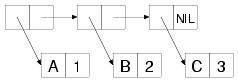
\includegraphics[scale=0.6]{images/alist-abc-123.png}
\end{figure}

Если значение \lstinline{CDR} не является списком, то cons-ячейки, представляющие пары ключ/значение,
будут \textit{точечными парами} (\textit{dotted pairs}) в терминах s-выражений. Ассоциативный
список, представленный на предыдущей диаграмме, к примеру, будет напечатан вот так:

\begin{myverb}
((A . 1) (B . 2) (C . 3))
\end{myverb}

Главная процедура поиска для ассоциативных списков~-- это \lstinline{ASSOC}, которая принимает
ключ и ассоциативный список в качестве аргументов и возвращает первую cons-ячейку, чей
\lstinline{CAR} соответствует ключу или является \lstinline{NIL}, если совпадения не найдено.
  
\begin{myverb}
CL-USER> (assoc 'a '((a . 1) (b . 2) (c . 3)))
(A . 1)
CL-USER> (assoc 'c '((a . 1) (b . 2) (c . 3)))
(C . 3)
CL-USER> (assoc 'd '((a . 1) (b . 2) (c . 3)))
NIL
\end{myverb}

Чтобы получить значение, соответствующее заданному ключу, вам следует просто передать
результат \lstinline{ASSOC} \lstinline{СDR}'у.
  
\begin{myverb}
CL-USER> (cdr (assoc 'a '((a . 1) (b . 2) (c . 3))))
1
\end{myverb}

По умолчанию заданный ключ сравнивается с ключами в ассоциативном списке, используя
предикат \lstinline{EQL}, но вы можете изменить его с помощью стандартной комбинации из
именованных аргументов \lstinline{:key} и \lstinline{:test}. Например, если вы хотите использовать
строковые ключи, то можете написать так:
  
\begin{myverb}
CL-USER> (assoc "a" '(("a" . 1) ("b" . 2) ("c" . 3)) :test #'string=)
("a" . 1)
\end{myverb}

Без явного задания в качестве \lstinline{:test} предиката \lstinline{STRING=} \lstinline{ASSOC}, вероятно,
вернул бы \lstinline{NIL}, потому что две строки с одинаковым содержимым необязательно равны
относительно \lstinline{EQL}.

\begin{myverb}
CL-USER> (assoc "a" '(("a" . 1) ("b" . 2) ("c" . 3)))
NIL
\end{myverb}

Поскольку при поиске \lstinline{ASSOC} просматривает список с начала, одна пара ключ/значение в
ассоциативном списке может скрывать другие пары с тем же ключом, но находящиеся дальше в
списке.

\begin{myverb}
CL-USER> (assoc 'a '((a . 10) (a . 1) (b . 2) (c . 3)))
(A . 10)
\end{myverb}

Вы можете добавить пару в начало списка с помощью функции \lstinline{CONS}, как здесь:

\begin{myverb}
(cons (cons 'new-key 'new-value) alist)
\end{myverb}

Однако для удобства Common Lisp предоставляет функцию \lstinline{ACONS}, которая позволяет вам
написать так:

\begin{myverb}
(acons 'new-key 'new-value alist)
\end{myverb}

Подобно \lstinline{CONS}, \lstinline{ACONS} является функцией и, следовательно, не может
модифицировать место, откуда был передан исходный ассоциативный список. Если вы хотите
модифицировать ассоциативный список, вам нужно написать так:

\begin{myverb}
(setf alist (acons 'new-key 'new-value alist))
\end{myverb}

\noindent{}или так:

\begin{myverb}
(push (cons 'new-key 'new-value) alist)
\end{myverb}

Очевидно, время, затраченное на поиск в ассоциативном списке при использовании
\lstinline{ASSOC}, является функцией от того, насколько глубоко в списке находится
соответствующая пара. В~худшем случае для определения, что никакая пара не соответствует
искомой, \lstinline{ASSOC} требуется просмотреть каждый элемент списка. Тем не менее поскольку
основной механизм работы ассоциативных списков довольно прост, то на небольших таблицах
ассоциативный список может превзойти в производительности хэш-таблицу.  Также
ассоциативные списки могут дать вам большую гибкость при выполнении поиска. Ранее я
отмечал, что \lstinline{ASSOC} принимает именованные аргументы \lstinline{:key} и \lstinline{:test}. Если
они не соответствуют вашим требованиям, вы можете использовать функции \lstinline{ASSOC-IF} и
\lstinline{ASSOC-IF-NOT}, которые возвращают первую пару ключ/значение, чей \lstinline{CAR}
удовлетворяет (или не удовлетворяет, в случае \lstinline{ASSOC-IF-NOT}) предикату,
передаваемому вместо ключа. Ещё три функции~-- \lstinline{RASSOC}, \lstinline{RASSOC-IF} и
\lstinline{RASSOC-IF-NOT}~-- действуют так же, как и соответствующие аналогичные
\lstinline{ASSOC}-функции, за исключением того, что они используют значение в \lstinline{CDR}
каждого элемента как ключ, совершая обратный поиск.

Функция \lstinline{COPY-ALIST} похожа на \lstinline{COPY-TREE}, за исключением того, что вместо
копирования всей древовидной структуры она копирует только те cons-ячейки, которые
составляют списочную структуру, плюс те cons-ячейки, на которые ссылаются \lstinline{CAR}'ы
этих ячеек. Другими словами, исходный ассоциативный список и его копия будут оба содержать
одинаковые объекты как в виде ключей, так и значений, даже если ключи или значения будут
состоять из cons-ячеек.

Наконец, вы можете создать ассоциативный список из двух различных списков ключей и значений
с помощью функции \lstinline{PAIRLIS}. Получившийся ассоциативный список может содержать пары
либо в том порядке, в каком они были в исходных списках, либо в обратном
порядке. Например, вы можете получить такой результат:

\begin{myverb}
CL-USER> (pairlis '(a b c) '(1 2 3))
((C . 3) (B . 2) (A . 1))
\end{myverb}

Или вы можете получить следующее:

\begin{myverb}
CL-USER> (pairlis '(a b c) '(1 2 3))
((A . 1) (B . 2) (C . 3))
\end{myverb}

Другой разновидностью таблицы поиска является список свойств (property list или сокращённо
plist), который вы использовали для представления строк базы данных в главе~\ref{ch:03}.
Структурно список свойств есть просто обычный список с ключами и значениями в виде
чередующихся величин. К примеру, список свойств, отображающий \lstinline{A}, \lstinline{B} и
\lstinline{C} на \lstinline{1}, \lstinline{2} и \lstinline{3},~-- это просто список \lstinline{(A 1 B 2 C 3)}. На
стрелочной диаграмме он выглядит так:

\begin{figure}[h]
  \centering
  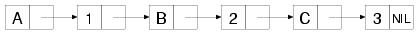
\includegraphics[scale=0.6]{images/plist-abc-123.png}
\end{figure}

Впрочем, списки свойств являются менее гибкими, чем ассоциативные списки. В
действительности список свойств поддерживает только одну фундаментальную операцию поиска,
функцию \lstinline{GETF}, которая принимает список свойств и ключ и возвращает связанное с
ключом значение или \lstinline{NIL}, если ключ не найден. \lstinline{GETF} также принимает
необязательный третий аргумент, который возвращается вместо \lstinline{NIL}, если ключ не
найден.

В~отличие от \lstinline{ASSOC}, которая использует \lstinline{EQL} как проверочный предикат по
умолчанию и позволяет использовать другой проверочный предикат в виде именованного
аргумента \lstinline{:test}, \lstinline{GETF} всегда использует \lstinline{EQ} для проверки, совпадает ли
переданный ей ключ с ключами списка свойств. Следовательно, вам никогда не следует
применять числа или знаки в качестве ключей в списке свойств; как вы видели в
главе~\ref{ch:04}, поведение \lstinline{EQ} для этих типов данных фактически не определено. На
практике ключи в списке свойств почти всегда являются символами, с тех пор как списки
свойств были впервые изобретены для реализации <<свойств>> символов, то есть произвольных
отображений между именами и значениями.

Вы можете использовать \lstinline{SETF} вместе с \lstinline{GETF} для установки переменной с
заданным ключом. \lstinline{SETF} также обращается с \lstinline{GETF} немного особым образом, при
котором первый аргумент \lstinline{GETF} считается модифицируемым. Таким образом, вы можете
вызвать \lstinline{SETF} поверх \lstinline{GETF} для добавления новых пар ключ/значение к
существующему списку свойств.
  
\begin{myverb}
CL-USER> (defparameter *plist* ())
*PLIST*
CL-USER> *plist*
NIL
CL-USER> (setf (getf *plist* :a) 1)
1
CL-USER> *plist*
(:A 1)
CL-USER> (setf (getf *plist* :a) 2)
2
CL-USER> *plist*
(:A 2)
\end{myverb}

Чтобы удалить пару ключ/значение из списка свойств, вы можете использовать макрос
\lstinline{REMF}, который присваивает месту, переданному в качестве своего первого аргумента,
список свойств, содержащий все пары ключ/значение, за исключением заданной. Он возвращает
истину, если заданный ключ был найден.
  
\begin{myverb}
CL-USER> (remf *plist* :a)
T
CL-USER> *plist*
NIL
\end{myverb}

Как и \lstinline{GETF}, \lstinline{REMF} всегда использует \lstinline{EQ} для сравнения заданного ключа с
ключами в списке свойств.

Поскольку списки свойств часто используются в ситуациях, когда вы хотите извлечь несколько
значений свойств из одного и того же списка, Common Lisp предоставляет функцию
\lstinline{GET-PROPERTIES}, которая делает более эффективным извлечение нескольких значений из
одного списка свойств. Она принимает список свойств и список ключей для поиска и
возвращает, в виде множества значений (\textit{multiple values}), первый найденный ключ,
соответствующее ему значение и голову списка, начинающегося с этого ключа. Это позволяет
вам обработать список свойств, извлекая из него нужные свойства, без продолжительного
повторного поиска с начала списка.  К примеру, следующая функция эффективно обрабатывает,
используя гипотетическую функцию \lstinline{process-property}, все пары ключ/значение в списке
свойств для заданного списка ключей:

\begin{myverb}
(defun process-properties (plist keys)
  (loop while plist do
	(multiple-value-bind (key value tail) (get-properties plist keys)
	  (when key (process-property key value))
	  (setf plist (cddr tail)))))
\end{myverb}

Последней особенностью списков свойств является их отношение к символам: каждый
символический объект имеет связанный список свойств, который может быть использован для
хранения информации о символе. Список свойств может быть получен с помощью функции
\lstinline{SYMBOL-PLIST}. Тем не менее обычно вам редко необходим весь список свойств; чаще вы
будете использовать функцию \lstinline{GET}, которая принимает символ и ключ и выполняет роль
сокращённой записи для \lstinline{GETF} с аргументами в виде того же ключа и списка символов,
возвращаемого \lstinline{SYMBOL-PLIST}.

\begin{myverb}
(get 'symbol 'key) === (getf (symbol-plist 'symbol) 'key)
\end{myverb}

Как с \lstinline{GETF}, к возвращаемому значению \lstinline{GET} можно применить \lstinline{SETF}, так
что вы можете присоединить произвольную информацию к символу, как здесь:

\begin{myverb}
(setf (get 'some-symbol 'my-key) "information")
\end{myverb}

Чтобы удалить свойство из списка свойств символа, вы можете использовать либо \lstinline{REMF}
поверх \lstinline{SYMBOL-PLIST}, либо удобную функцию \lstinline{REMPROP}\footnote{Также возможно
  напрямую выполнить \lstinline{SETF} над значением, возвращаемым \lstinline{SYMBOL-PLIST}. Однако
  это плохая идея, поскольку различный код может добавлять различные свойства к символам
  списка свойств с разными целями. Если один кусок кода затирает весь список свойств
  символа, он может помешать работе другого кода, который добавил свои свойства к списку.}.

\begin{myverb}
(remprop 'symbol 'key) === (remf (symbol-plist 'symbol) 'key)
\end{myverb}

Возможность связывать произвольную информацию с именами довольно удобна, если вы
занимаетесь какого-либо рода символическим программированием. К примеру, один макрос,
который вы напишете в главе~\ref{ch:24}, будет связывать информацию с именами, которую
другие экземпляры того же макроса будут извлекать и использовать при собственном
раскрытии.

\section{DESTRUCTURING-BIND}

Последний инструмент для разделки и нарезки списков, о котором я должен рассказать,
поскольку он понадобится вам в дальнейших главах,~-- это макрос
\lstinline{DESTRUCTURING-BIND}. Этот макрос предоставляет способ \textit{деструктурировать}
(\textit{destructure}) произвольные списки, подобно тому как списки параметров макроса
могут разбирать на части свои списки аргументов. Основной скелет \lstinline{DESTRUCTURING-BIND}
таков:

\begin{myverb}
(destructuring-bind (parameter*) list
  body-form*)
\end{myverb}

Список параметров может включать любые из типов параметров, поддерживаемых в списках
параметров макросов, таких как \lstinline!&optional!, \lstinline!&rest! и
\lstinline!&key!\footnote{Списки параметров макроса поддерживают один тип параметра,
  который не поддерживает \lstinline{DESTRUCTURING-BIND},~-- это \lstinline!&environment!. Тем не
  менее я не обсуждал этот тип параметра в главе~\ref{ch:08}, и сейчас вам не стоит об
  этом беспокоиться.}. Как и в списке параметров макроса, любой параметр может быть заменён
на вложенный деструктурирующий список параметров, который разделяет список на составные
части, иначе список целиком был бы связан с заменённым параметром. Форма \textit{list}
вычисляется один раз и возвращает список, который затем деструктурируется, и
соответствующие значения связываются с переменными в списке параметров. Затем по порядку
вычисляются все \textit{body-form} с учётом значений связанных переменных. Вот несколько
простых примеров:
  
\begin{myverb}
(destructuring-bind (x y z) (list 1 2 3)
(list :x x :y y :z z)) ==> (:X 1 :Y 2 :Z 3)

(destructuring-bind (x y z) (list 1 (list 2 20) 3)
(list :x x :y y :z z)) ==> (:X 1 :Y (2 20) :Z 3)

(destructuring-bind (x (y1 y2) z) (list 1 (list 2 20) 3)
(list :x x :y1 y1 :y2 y2 :z z)) ==> (:X 1 :Y1 2 :Y2 20 :Z 3)

(destructuring-bind (x (y1 &optional y2) z) (list 1 (list 2 20) 3)
(list :x x :y1 y1 :y2 y2 :z z)) ==> (:X 1 :Y1 2 :Y2 20 :Z 3)

(destructuring-bind (x (y1 &optional y2) z) (list 1 (list 2) 3)
(list :x x :y1 y1 :y2 y2 :z z)) ==> (:X 1 :Y1 2 :Y2 NIL :Z 3)

(destructuring-bind (&key x y z) (list :x 1 :y 2 :z 3)
(list :x x :y y :z z)) ==> (:X 1 :Y 2 :Z 3)

(destructuring-bind (&key x y z) (list :z 1 :y 2 :x 3)
(list :x x :y y :z z)) ==> (:X 3 :Y 2 :Z 1)
\end{myverb}

Единственный вид параметра, который вы можете использовать как с
\lstinline{DESTRUCTURING-BIND}, так и в списках параметров макросов, о котором я не упомянул в
главе~\ref{ch:08},~-- это параметр \lstinline!&whole!. Если он указан, то располагается
первым в списке параметров и связывается со всей формой списка целиком\footnote{Когда
  параметр \lstinline!&whole! используется в списке параметров макроса, то форма, с которой
  он связан, соответствует всей форме макроса, включая имя макроса.}. После параметра
\lstinline!&whole! другие параметры могут появляться как обычно и извлекать определённые
части списка, как если бы параметр \lstinline!&whole! отсутствовал. Пример использования
\lstinline!&whole! вместе с \lstinline{DESTRUCTURING-BIND} выглядит так:
  
\begin{myverb}
(destructuring-bind (&whole whole &key x y z) (list :z 1 :y 2 :x 3)
  (list :x x :y y :z z :whole whole))
==> (:X 3 :Y 2 :Z 1 :WHOLE (:Z 1 :Y 2 :X 3))
\end{myverb}

Вы будете использовать параметр \lstinline!&whole! в одном из макросов, составляющих часть
библиотеки для генерации HTML, которую вы разработаете в главе~\ref{ch:31}.  Однако мне
нужно рассмотреть ещё несколько вопросов, прежде чем вы приступите к ней. После двух глав
довольно лисповских тем про cons-ячейки вы можете перейти к более прозаичным вопросам о том,
как работать с файлами и именами файлов.


%%% Local Variables: 
%%% mode: latex
%%% TeX-master: "pcl-ru"
%%% TeX-open-quote: "<<"
%%% TeX-close-quote: ">>"
%%% End: 
